\documentclass[tikz, border=1cm]{standalone}

\usepackage{tikz}
\usetikzlibrary{calc}

\begin{document}
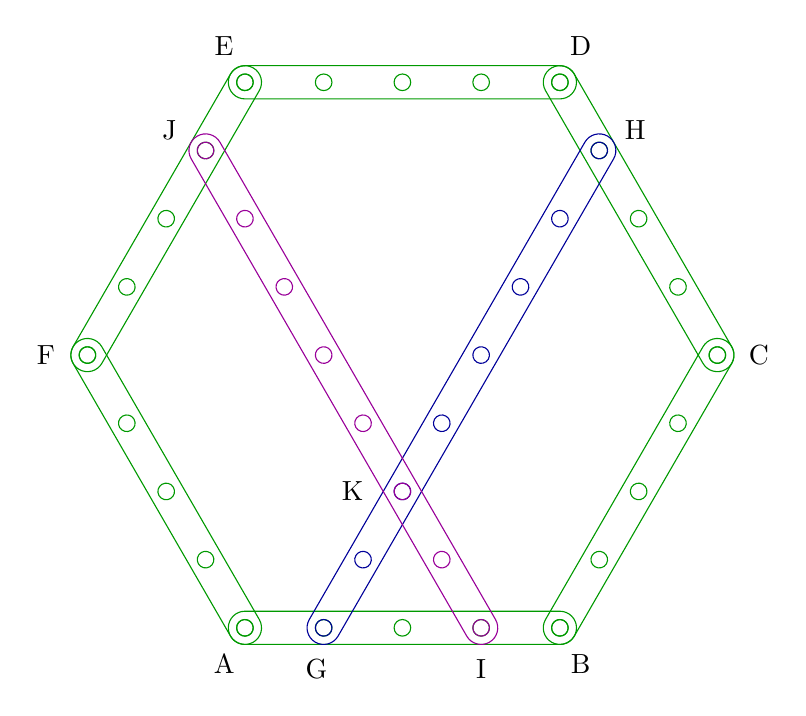
\begin{tikzpicture}

\newcommand{\rod}[4][000000] % [color][n][sep][prop]
{
 \definecolor{main}{HTML}{#1}
 \draw[main] (0,{{2*#4}})
   -- ++({#2*#3},0) arc(+90:-90:{2*#4})
   -- ++({-#2*#3},0) arc(270:90:{2*#4});
 \foreach \x in {0,1,...,#2}
  \draw[main] (\x,0) circle (#4);
}

\def\s {4} \def\f {1}
\def\p {3pt}
\begin{scope}
 \rod[009900]{\s}{\f}{\p} \path (0,0) ++(240:5*\p) node{A};
 \begin{scope}[shift={(\s,0)},rotate=60]
  \rod[009900]{\s}{\f}{\p} \path (0,0) ++(240:5*\p) node{B};
  \begin{scope}[shift={(\s,0)},rotate=60]
   \rod[009900]{\s}{\f}{\p} \path (0,0) ++(240:5*\p) node{C};
   \begin{scope}[shift={(\s,0)},rotate=60]
    \rod[009900]{\s}{\f}{\p} \path (0,0) ++(240:5*\p) node{D};
    \begin{scope}[shift={(\s,0)},rotate=60]
     \rod[009900]{\s}{\f}{\p} \path (0,0) ++(240:5*\p) node{E};
     \begin{scope}[shift={(\s,0)},rotate=60]
      \rod[009900]{\s}{\f}{\p} \path (0,0) ++(240:5*\p) node{F};
     \end{scope}
    \end{scope}
   \end{scope}
  \end{scope}
 \end{scope}
\end{scope}

\begin{scope}[shift={(1,0)},rotate=60]
 \rod[000099]{7}{1}{\p}
 \path (0,0) ++(200:5*\p) node{G};
 \path (7,0) ++(-30:5*\p) node{H};
\end{scope}

\begin{scope}[shift={(3,0)},rotate=120]
 \rod[990099]{7}{1}{\p}
 \path (0,0) ++(150:5*\p) node{I};
 \path (7,0) ++(30:5*\p) node{J};
 \path (2,0) ++(60:6*\p) node{K};
\end{scope}




\end{tikzpicture}
\end{document}
